\section{Cenário de Teste 3}

Este cenário está dividido em 5 (cinco) exemplos, os quais são apresentados a seguir, contemplando todo o processo de auto-localização
em cada exemplo, a partir da apresentação das Imagens abaixo.

\subsection{Exemplo 1}

Exemplo utilizando velocidade de deslocamento em 10 unidades de diâmetro por segundo:

\begin{figure}[H]
  \centering
  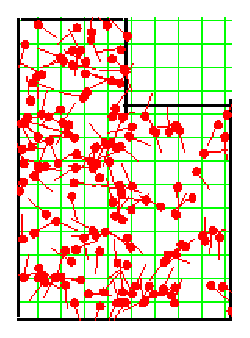
\includegraphics[scale=1]{figuras/cen3_ex1/1.eps}
  \caption[Partículas Iniciais]{Partículas iniciais}
  \label{img:cen3_ex1_1}
\end{figure}

\begin{figure}[H]
  \centering
  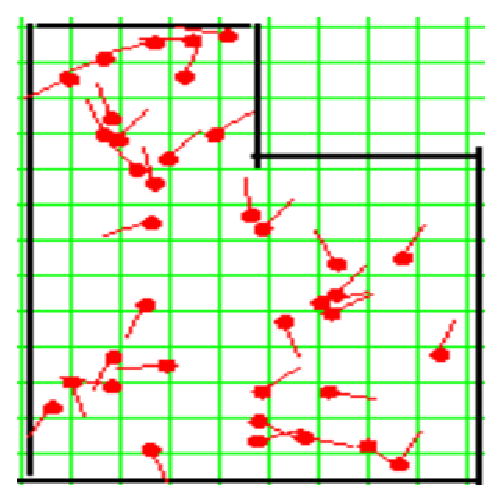
\includegraphics[scale=1]{figuras/cen3_ex1/2.eps}
  \caption[Primeiro Ciclo de Filtragem]{Primeiro ciclo de filtragem}
  \label{img:cen3_ex1_2}
\end{figure}

\begin{figure}[H]
  \centering
  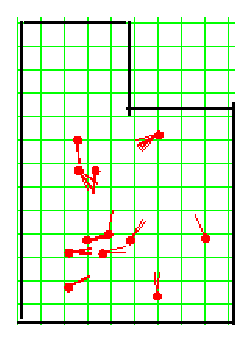
\includegraphics[scale=1]{figuras/cen3_ex1/3.eps}
  \caption[Segundo Ciclo de Filtragem]{Segundo ciclo de filtragem}
  \label{img:cen3_ex1_3}
\end{figure}

\begin{figure}[H]
  \centering
  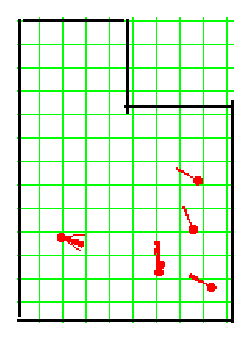
\includegraphics[scale=1]{figuras/cen3_ex1/4.eps}
  \caption[Terceiro Ciclo de Filtragem]{Terceiro ciclo de filtragem}
  \label{img:cen3_ex1_4}
\end{figure}

\begin{figure}[H]
  \centering
  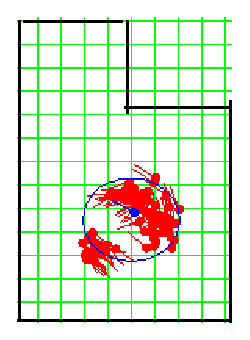
\includegraphics[scale=1]{figuras/cen3_ex1/5.eps}
  \caption[Quarto Ciclo de Filtragem]{Quarto ciclo de filtragem}
  \label{img:cen3_ex1_5}
\end{figure}

\begin{figure}[H]
  \centering
  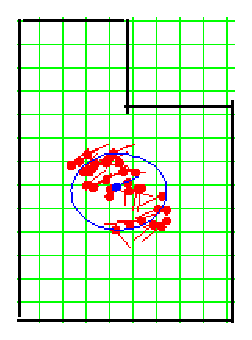
\includegraphics[scale=1]{figuras/cen3_ex1/6.eps}
  \caption[Quinto Ciclo de Filtragem]{Quinto ciclo de filtragem}
  \label{img:cen3_ex1_6}
\end{figure}

\begin{figure}[H]
  \centering
  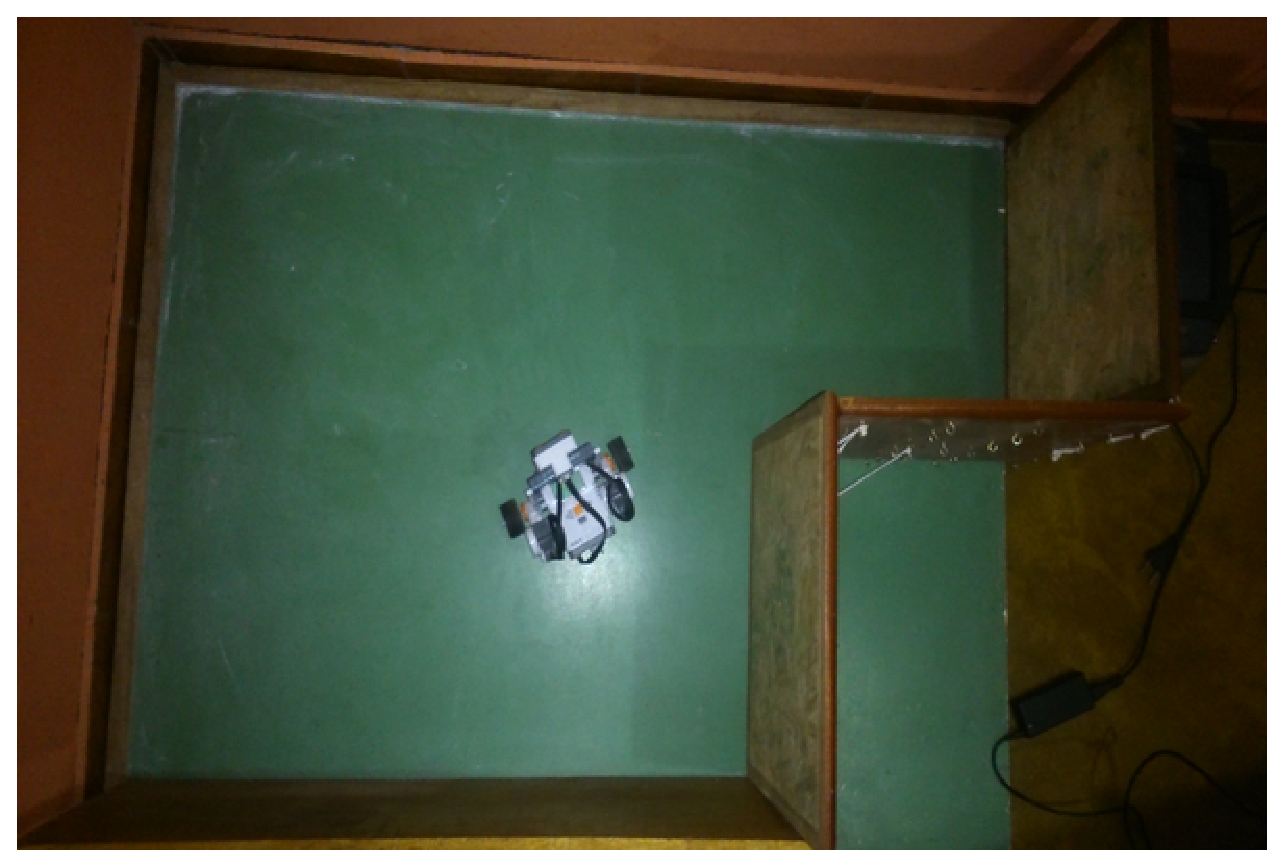
\includegraphics[scale=1]{figuras/cen3_ex1/real.eps}
  \caption[Posição Real do Robô]{Posição Real do Robô.}
  \label{img:cen3_ex1_real}
\end{figure}
